\chapter{Measuring Capacitance}

In order to measure the capacitance of the capacitors without using the "capacitance" function on the digital multimeter, we have used the circuit shown in Figure \ref{fig:capacitance-circuit}:

\begin{figure}[h]
    \centering
    \begin{circuitikz} \draw
        (0,0) to[square voltage source, l=0-5V] (0,4)
        to[R, l=$5k\Omega$] (4,4) 
        to[C, l=C] (4,0) -- (0,0)
        ;
        \end{circuitikz}
    \caption{Circuit to Measure Capacitance}
    \label{fig:capacitance-circuit}
\end{figure}

The circuit consists of a square wave voltage source @ 5V zero-to-peak, a 5k$\Omega$ resistor and a capacitor. The voltage across the capacitor is measured using the oscilloscope. The time taken for the voltage to reach 63.2\% of the maximum voltage is measured. The capacitance is then calculated using the formula:

\begin{align*}
    &V(t) = V_{\max} \cdot e^{-\frac{t}{RC}} \\
    &\boxed{C = \frac{t}{R}}
\end{align*}

Where:
\begin{itemize}
    \item C is the capacitance in Farads
    \item t is the time taken for the voltage to reach 63.2\% of the maximum voltage in seconds
    \item R is the resistance in Ohms
\end{itemize}

\newpage
\thispagestyle{plain}

\section{Theoretical Analysis}
We have decided to use this circuit to measure the capacitance of the capacitors. The circuit is shown in Figure \ref{fig:capacitance-circuit}. First, we tested if the circuit is working by trying everything in LTSpice:

\begin{figure}[h]
    \centering
    \includegraphics[width=0.8\textwidth]{assets/1714061123.png}
    \caption{LTSpice Simulation of the Circuit}
    \label{fig:ltspice-simulation}
\end{figure}

We have theoretically calculated the capacitance of our capacitor and compared the results from the simulation and the theoretical calculations.


\begin{table}[h]
    \centering
    \begin{tabular}{l|l|l|}
    \cline{2-3}
                                                            & $\epsilon_r$ & Theoretical Capacitance \\ \hline
    \multicolumn{1}{|l|}{PLA \textbackslash{}w 75\% Infill} & 2.4     & 1.3nF                       \\ \hline
    \multicolumn{1}{|l|}{PLA \textbackslash{}w 15\% Infill} & 0.48    & 0.26nF                \\ \hline
    \multicolumn{1}{|l|}{Cylindirical} & 1 (Empty)    & 43pF                  \\ \hline
    \end{tabular}
    \caption{Theoretical Capacitance Values}
\end{table}

And after checking the results from the simulation, we have seen that the results are very close to the theoretical calculations ($\pm10\%$). Therefore, we have decided to use this circuit to measure the capacitance of the capacitors.


\newpage{}
\thispagestyle{plain}

\section{Results}

We have measured the time taken for the voltage to reach 63.2\% of the maximum voltage using the oscilloscope because after $RC$ seconds later the voltage reachs this value. Table \ref{fig:time-taken} shows the time taken for the voltage to reach 63.2\% of the maximum voltage for the capacitors:

\begin{center}
    \begin{table}[h]
        \centering
            \begin{tabular}{l|l|l|l|}
            \cline{2-4}
                                    & Cylindirical & Parallel \textbackslash{}w 75\% Infill & Parallel \textbackslash{}w 15\% Infill \\ \hline
            \multicolumn{1}{|l|}{t} & $200\mu s$          & $7ms$                                   & $2ms$                                     \\ \hline
            \end{tabular}
        \caption{Time Taken for Voltage to Reach 63.2\% of Maximum Voltage}
        \label{fig:time-taken}
        \end{table}
\end{center}

The resistance used in the circuit is 5k$\Omega$. Using the formula mentioned above, the capacitance of the capacitors is calculated as follows:

\begin{align*}
    C_{cylindrical} &= \frac{200\mu s}{5k\Omega} = \boxed{40pF} \\
    C_{parallel~75\%~Infill} &= \frac{7ms}{5k\Omega} = \boxed{1.4nF} \\
    C_{parallel~15\%~Infill} &= \frac{2ms}{5k\Omega} = \boxed{0.4nF}
\end{align*}

\section{Comparing Simulation \& Measurement Results}

The capacitance of the capacitors is calculated using circuit shown in Figure \ref{fig:capacitance-circuit} and the formula mentioned above. We have set the circuit up and measured time values of the capacitors:

\begin{figure}[h]
    \centering
    \includegraphics[width=0.6\textwidth]{assets/2WhatsApp Image 2024-04-18 at 20.32.11.jpeg}
    \caption{Circuit Setup}
    \label{fig:circuit-setup}
\end{figure}

\newpage
\thispagestyle{plain}

We can easily see the charging and discharging of the capacitor in the oscilloscope:

\begin{figure}[h]
    \centering
    \includegraphics[width=0.6\textwidth]{assets/WhatsApp Image 2024-04-16 at 18.20.12 (2).jpeg}
    \caption{Oscilloscope Results}
    \label{fig:oscilloscope-results}
\end{figure}

The same circuit is simulated using LTSpice. The simulation results are shown in Figure \ref{fig:ltspice-simulation}:

\begin{figure}[h]
    \centering
    \includegraphics[width=0.8\textwidth]{assets/1714059734.png}
    \caption{LTSpice Simulation Results}
    \label{fig:ltspice-simulation}
\end{figure}

We can easily see the charging and discharging of the capacitor in the simulation results. 

If we compare the simulation and the measurement results, we can see that the results are very close to each other. The capacitance values are calculated as follows:

\begin{table}[h]
    \centering
    \begin{tabular}{l|l|l|}
    \cline{2-3}
                                                            & Simulation & Measurement \\ \hline
    \multicolumn{1}{|l|}{PLA \textbackslash{}w 75\% Infill} & 1.3nF     & 1.4nF      \\ \hline
    \multicolumn{1}{|l|}{PLA \textbackslash{}w 15\% Infill} & 0.26nF    & 0.4nF      \\ \hline
    \multicolumn{1}{|l|}{Cylindirical} & 43pF     & 40pF       \\ \hline
    \end{tabular}
    \caption{Simulation \& Measurement Results}
\end{table}



\newpage
\thispagestyle{plain}

\section{Variation of Capacitance}

Our designed capacitors are variable capacitors and their capacitance values can be changed. 

\subsection{Parallel Plate Capacitors}

For parallel plate capacitor, we can calculate the capacitance with the following equation:

\begin{align*}
    C &= \varepsilon\cdot\frac{A}{d}
\end{align*}

Where:
\begin{itemize}
    \item C is the capacitance in Farads
    \item $\varepsilon$ is the permittivity of the dielectric material in Farads per meter ($\varepsilon_0\varepsilon_r$)
    \item A is the area of the plates in square meters
    \item d is the separation between the plates in meters
\end{itemize}

The capacitance of the parallel plate capacitor can be changed by changing any value in the equation. We have decided to change $\varepsilon~(=\varepsilon_0\cdot\boxed{\varepsilon_r})$ value by varying the infill density of the plates.
The capacitance of the parallel plate capacitor is directly proportional to the permittivity of the dielectric material. The capacitance of the capacitor with 75\% infill density is higher because the permittivity of the dielectric material is higher. 

\begin{figure}[h]
    \centering
    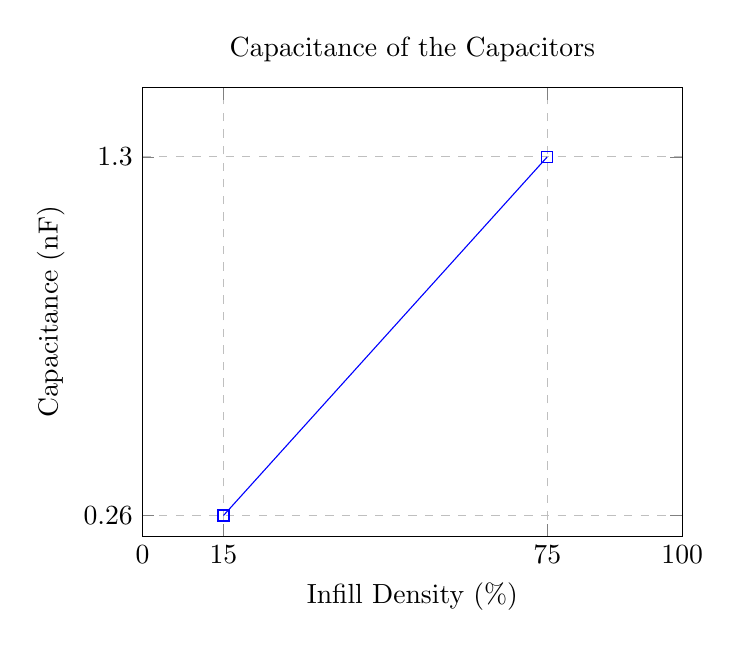
\begin{tikzpicture}
        \begin{axis}[
            title={Capacitance of the Capacitors},
            xlabel={Infill Density (\%)},
            ylabel={Capacitance (nF)},
            xmin=0, xmax=1,
            ymin=0.2, ymax=1.5,
            xtick={0, 0.15, 0.75, 1},
            ytick={0, 0.26, 1.3},
            xticklabels={0, 15, 75, 100},
            yticklabels={0, 0.26, 1.3},
            legend pos=north west,
            ymajorgrids=true,
            xmajorgrids=true,
            grid style=dashed,
        ]
        
        \addplot[
            color=blue,
            mark=square,
            ]
            coordinates {
            (0.15, 0.26)
            (0.75, 1.3)
            };
        
        \end{axis}
    \end{tikzpicture}
    \caption{Capacitance vs Infill Density Table}
    \label{fig:capacitance-plot}
\end{figure}

\newpage
\thispagestyle{plain}

\subsection{Cylindrical Capacitors}

For cylindrical capacitor, we can calculate the capacitance with the following equation:

\begin{align*}
    C &= 2\pi\varepsilon\frac{L}{\ln{\frac{r_2}{r_1}}}
\end{align*}

Where:
\begin{itemize}
    \item C is the capacitance in Farads
    \item $\varepsilon$ is the permittivity of the dielectric material in Farads per meter ($\varepsilon_0\varepsilon_r$)
    \item L is the length of the cylinder in meters
    \item $r_1$ is the inner radius of the cylinder in meters
    \item $r_2$ is the outer radius of the cylinder in meters
\end{itemize}

The capacitance of the cylindrical capacitor can be changed by changing any value in the equation. We have decided to change $L$ value by varying the height of the cylinder as shown in Figure \ref{fig:cylindirical-varying}. The capacitance of the cylindirical capacitor is directly proportional to length of the capacitor. The capacitance of the capacitor with 22cm height is higher than with 10cm height because the length of the capacitor is higher.

\begin{figure}[h]
    \centering
    \includegraphics[width=1\textwidth]{assets/cylindirical-variable.png}
    \caption{Cylindirical Capacitor Varying}
    \label{fig:cylindirical-varying}
\end{figure}

\newpage
\thispagestyle{plain}

We have made 5 different measurements for the cylindrical capacitor. Calculated the capacitance values using the same formula mentioned above ($C = \frac{t}{R}$). The capacitance values are shown in Figure \ref{fig:cylindirical-capacitance-plot}:

\begin{figure}[h]
    \centering
    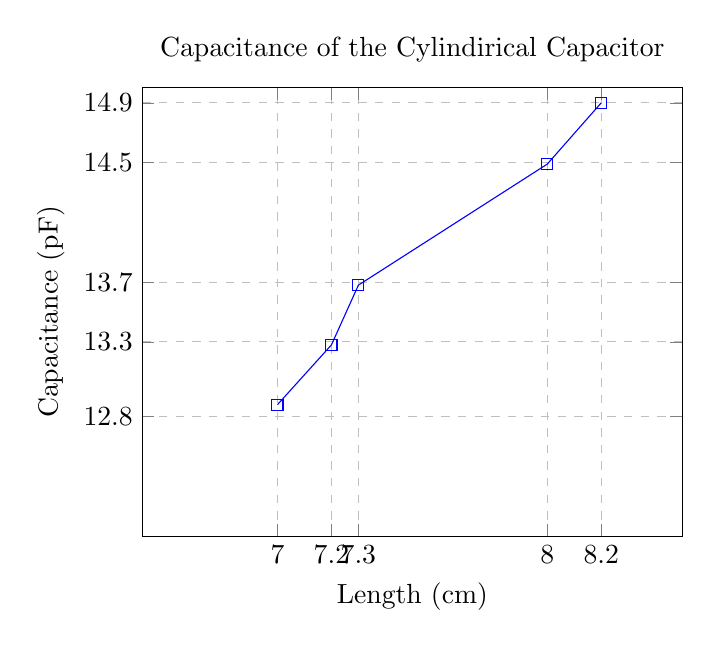
\begin{tikzpicture}
        \begin{axis}[
            title={Capacitance of the Cylindirical Capacitor},
            xlabel={Length (cm)},
            ylabel={Capacitance (pF)},
            xmin=6.5, xmax=8.5,
            ymin=12, ymax=15,
            legend pos=north west,
            ymajorgrids=true,
            xmajorgrids=true,
            grid style=dashed,
            xtick={7, 7.2, 7.3, 8, 8.2},
            ytick={12.8, 13.3, 13.7, 14.5, 14.9},
        ]
        
        \addplot[
            color=blue,
            mark=square,
            ]
            coordinates {
            (7, 12.88)
            (7.2, 13.28)
            (7.3, 13.68)
            (8, 14.49)
            (8.2, 14.9)
            };
        
        \end{axis}
    \end{tikzpicture}
    \caption{Capacitance vs Length Table}
    \label{fig:cylindirical-capacitance-plot}
\end{figure}
